\section{Grafi di assemblaggio}
La bioinformatica sta ancora cercando di capire in modo chiaro come siano fatti i nucleotidi del genoma umano. Il problema del sequenziamento umano fino a qualche decennio fa era troppo complicato, quindi i primi studi su organismi più semplici come il lievito o i moscerini della frutta.

L'assemblaggio dei genomi è effettuata da porzioni di genoma definite \textit{read}, di 50-10.000$bp$ (base pairs). Questi spesso vengono in coppia (mate pairs), ma non è possibile identificarne la posizione originaria a partire dai singoli pezzi: da qui il problema della ricostruzione.

Per la costruzione, vengono utilizzati dei sequenziatori, che ottengono read a partire dal genoma sfruttandone le proprietà biochimiche. Il numero medio di read estratte è definito \textit{copertura}.

L'evoluzione tecnologica ha permesso sviluppi di attrezzature in grado di classificare read sempre più lunghi, in base ai gigabyte per run. Sanger è uno dei più importanti elaboratori che ha permesso di identificare i read prima del 2006, con costi elevatissimi. Il progresso nel campo dell'informatica ha portato a tempi e costi molto più brevi, ma ci sono altri importanti fattori da tenere in considerazione: il tasso di errore e la distribuzione dell'errore.

Il sistema che individua i read più lunghi (10.000) ha un tasso di errore di circa il 15\%, mentre altri hanno meno dell'1\textperthousand\ ma errori sistematici (che invalidano l'analisi). 

Per rimediare a questi problemi sono utilizzati agenti chimici (adattatori) che rendono il DNA più leggibile, tagliandolo in entrambi i lati. Le read si possono estrarre di una lunghezza relativamente bassa conoscendo la distanza tra ogni coppia di esse.

Il problema, in questo caso, è la ricostruzione del genoma di partenza a partire dalle read. Non è conosciuto il punto di inizio e di fine di esse nella stringa iniziale. 

C'è una proprietà che si può sfruttare: l'overlap. Il suffisso di una read può essere prefisso di un'altra read (sovrapposizione). Pezzi di sequenze uguali vengono quindi unite, ma questo causa ulteriori problemi:
\begin{enumerate}
	\item Casualità, se le sovrapposizioni sono brevi (quindi si è interessati solo a quelle sufficientemente lunghe);
	\item Errore nella lettura;
	\item Organismi diploidi (come l'uomo), con una copia del genoma di ogni genitore che comportano sequenze con piccole differenze (SNIP, Single Nucleotide Polymorphism).
\end{enumerate}

\begin{example}{}{}

$$\begin{matrix}
	T & C & T & A & T & A & T & C & T & C & G & G & C & T & C & T & A & G & G & ~ & ~ \\
	~ & ~ & ~ & ~ & | & | & | & | & | & | & | & ~ & | & | & | & | & | & | & | & ~ & ~ \\
	~ & ~ & ~ & ~ & T & A & T & C & T & C & G & A & C & T & C & T & A & G & G & C & C
\end{matrix}$$

Probabile motivo:

$$
\begin{matrix}
	~ & ~ & ~ & ~ & C & T & A & T & A & T & C & T & C & G & G & C & T & ~ & \\
	G & C & G & T & C & T & A & T & A & T & C & T & C & G & G & C & T & C & T & A & G & G & C \\
	~ & ~ & ~ & ~ & ~ & ~ & ~ & ~ & A & T & C & T & C & G & \textcolor{red}{A} & C & T & C & T
\end{matrix}
$$

\end{example}

\subsection{Shortest superstring}
Questo problema è una semplificazione della ricostruzione del genoma, che non lo gestisce interamente ma ha in comune molti elementi. 

Dato un insieme $S = \{s_1,\ \dots,\ s_n\}$ di stringhe, trovare una stringa $T$ tale che ogni stringa $s_i$ è sottostringa di $T$.

Applicando questo problema alle read, la funzione obiettivo è $|T|$, $T$ rappresenta il genoma assemblato e $S$ le read. Bisogna però gestire le regioni ripetute, ovvero tenere conto della possibilità di grandi regioni quasi uguali.

Una risoluzione greedy consiste nel fondere le due stringhe con massimo overlap iterativamente finché non ne rimane una sola. Tanto più lunghe sono le read, tanto più lunghe saranno le sottosequenze che è possibile distinguere.

Esempio: \textbf{a\_long\_long\_long\_time}

\begin{enumerate}
	\item ng\_lon \_long\_ a\_long long\_l ong\_ti ong\_lo long\_t g\_long g\_time \textbf{ng\_tim}
	\item ng\_time ng\_lon \textbf{\_long\_} a\_long long\_l ong\_ti ong\_lo long\_t \textbf{g\_long}
	\item ng\_time g\_long\_ ng\_lon a\_long long\_l \textbf{ong\_ti} ong\_lo \textbf{long\_t}
	\item ng\_time long\_ti g\_long\_ \textbf{ng\_lon} a\_long long\_l \textbf{ong\_lo}
	\item \textbf{ng\_time} ong\_lon \textbf{long\_ti} g\_long\_ a\_long long\_l
	\item \textbf{ong\_lon} long\_time g\_long\_ a\_long long\_l
	\item long\_lon \textbf{long\_time} \textbf{g\_long\_} a\_long
	\item \textbf{long\_lon} \textbf{g\_long\_time} a\_long
	\item \textbf{long\_long\_time} \textbf{a\_long}
	\item a\_long\_long\_time
\end{enumerate}

L'algoritmo è NP-hard, e dato che ci sono porzioni quasi perfettamente ripetute (duplicazione), ci saranno regioni estremamente simili che verranno prese in considerazione solo una volta.

\newpage
\section{String graph per l'assemblaggio}
Il problema di assemblaggio del genoma, quindi, è ridotto a un problema su grafi. Ogni read corrisponde a un vertice, e i collegamenti sono rappresentati tramite archi con un'etichetta che ne indica la lunghezza. Le rappresentazioni più comuni sono \textbf{OLC} e \textbf{De Bruijn}.

Ogni superstringa viene convertita in un grafo completo, orientato e pesato. Data una funzione $ov$ che calcola l'overlap (orientato), ogni etichetta è ottenuta con $|A| - ov(A, B)$ con $A$ nodo di partenza, $B$ nodo di arrivo. Si vuole trovare il cammino più corto che tocca ogni vertice una e una sola volta.

Considerando che il genoma umano è formato da 4 nucleotidi in una struttura a doppia elica, secondo la legge di Watson-Crick si ha $A \leftrightarrow T$ e $C \leftrightarrow G$: i due filamenti sono uno il complemento dell'altro. Fra una coppia di vertici si potrebbe avere fino a 4 archi, di cui due riferiti al \textit{reverse and complement}. Per ridurre questo problema ci sono tecniche euristiche.

\subsection{Grafi di overlap}
Un grafo di overlap è una rappresentazione astratta in cui ogni read è un nodo, e se l'overlap è \textit{abbastanza lungo} i nodi sono collegati con un arco. L'etichetta di ogni arco è la parte che precede la sovrapposizione. 

Tutte le possibili sovrapposizioni sono rappresentate, ma la stringa di partenza va ricostruita in modo preciso tramite visita del grafo in base alla lunghezza dell'etichetta. Alcuni archi, però, non sono informativi (stringhe non consecutive), e per questo motivo essi vengono rimossi.

\tikzset{every picture/.style={line width=0.75pt}} %set default line width to 0.75pt        
\begin{figure}[H]
\caption{Grafo di Overlap}
\begin{center}
Read: \texttt{ACGTGTG}, \texttt{CGTGTGC}, \texttt{GTGCCA}, \texttt{CCACG}
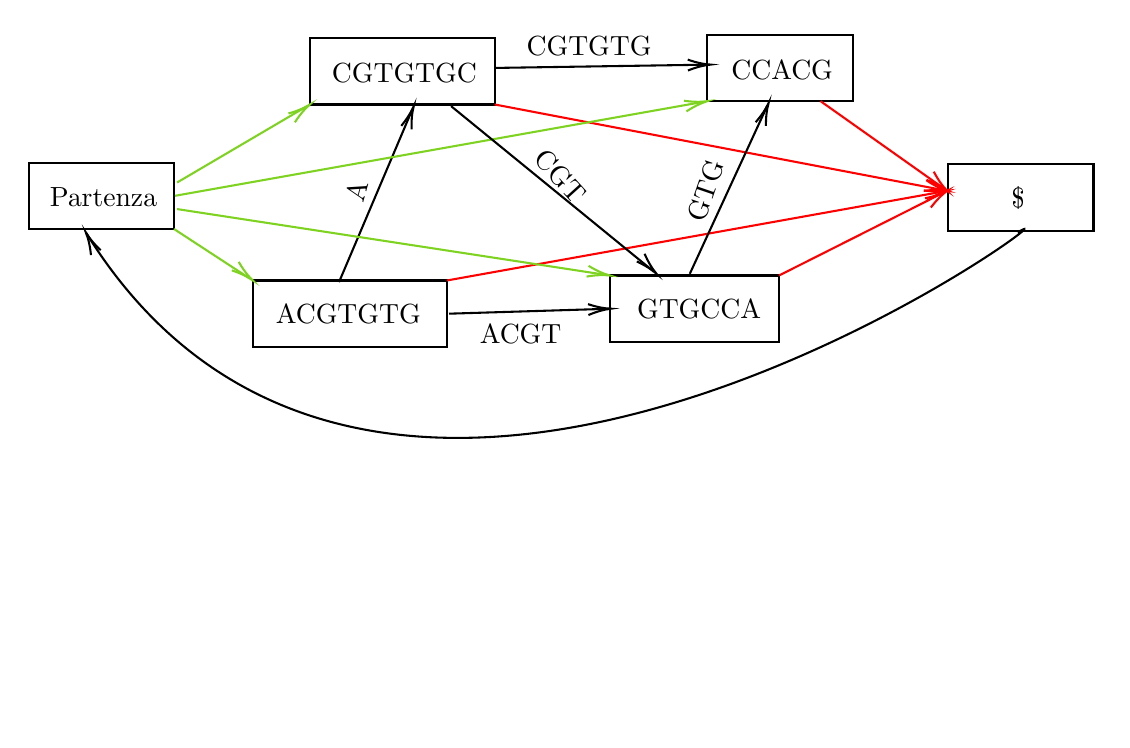
\begin{tikzpicture}[x=0.75pt,y=0.6pt,yscale=-1,xscale=1]
%uncomment if require: \path (0,281); %set diagram left start at 0, and has height of 281
%Shape: Rectangle [id:dp6560992130069507] 
\draw   (158.5,30) -- (247.5,30) -- (247.5,70) -- (158.5,70) -- cycle ;
%Shape: Rectangle [id:dp8633094909301302] 
\draw   (350,28) -- (420,28) -- (420,68) -- (350,68) -- cycle ;
%Straight Lines [id:da17421981355945193] 
\draw    (247.5,48) -- (349.5,46.04) ;
\draw [shift={(351.5,46)}, rotate = 538.9] [color={rgb, 255:red, 0; green, 0; blue, 0 }  ][line width=0.75]    (10.93,-3.29) .. controls (6.95,-1.4) and (3.31,-0.3) .. (0,0) .. controls (3.31,0.3) and (6.95,1.4) .. (10.93,3.29)   ;

%Shape: Rectangle [id:dp26552417711503384] 
\draw   (131,176) -- (224.5,176) -- (224.5,216) -- (131,216) -- cycle ;
%Shape: Rectangle [id:dp10524493499981546] 
\draw   (303,173) -- (384.5,173) -- (384.5,213) -- (303,213) -- cycle ;
%Straight Lines [id:da8474295750375322] 
\draw    (172.5,177) -- (207.86,72.89) ;
\draw [shift={(208.5,71)}, rotate = 468.76] [color={rgb, 255:red, 0; green, 0; blue, 0 }  ][line width=0.75]    (10.93,-3.29) .. controls (6.95,-1.4) and (3.31,-0.3) .. (0,0) .. controls (3.31,0.3) and (6.95,1.4) .. (10.93,3.29)   ;

%Straight Lines [id:da7595524463463148] 
\draw    (225.5,196) -- (301.5,193.08) ;
\draw [shift={(303.5,193)}, rotate = 537.8] [color={rgb, 255:red, 0; green, 0; blue, 0 }  ][line width=0.75]    (10.93,-3.29) .. controls (6.95,-1.4) and (3.31,-0.3) .. (0,0) .. controls (3.31,0.3) and (6.95,1.4) .. (10.93,3.29)   ;

%Shape: Rectangle [id:dp375619585347468] 
\draw   (466,106) -- (536,106) -- (536,146) -- (466,146) -- cycle ;
%Straight Lines [id:da8048124855752778] 
\draw [color={rgb, 255:red, 255; green, 0; blue, 0 }  ,draw opacity=1 ]   (404.5,68) -- (464,120.67) ;
\draw [shift={(465.5,122)}, rotate = 221.52] [color={rgb, 255:red, 255; green, 0; blue, 0 }  ,draw opacity=1 ][line width=0.75]    (10.93,-3.29) .. controls (6.95,-1.4) and (3.31,-0.3) .. (0,0) .. controls (3.31,0.3) and (6.95,1.4) .. (10.93,3.29)   ;

%Straight Lines [id:da91205814003782] 
\draw [color={rgb, 255:red, 255; green, 0; blue, 0 }  ,draw opacity=1 ]   (384.5,173) -- (463.81,123.07) ;
\draw [shift={(465.5,122)}, rotate = 507.8] [color={rgb, 255:red, 255; green, 0; blue, 0 }  ,draw opacity=1 ][line width=0.75]    (10.93,-3.29) .. controls (6.95,-1.4) and (3.31,-0.3) .. (0,0) .. controls (3.31,0.3) and (6.95,1.4) .. (10.93,3.29)   ;

%Straight Lines [id:da9132525115334023] 
\draw [color={rgb, 255:red, 255; green, 0; blue, 0 }  ,draw opacity=1 ]   (224.5,176) -- (463.55,122.44) ;
\draw [shift={(465.5,122)}, rotate = 527.37] [color={rgb, 255:red, 255; green, 0; blue, 0 }  ,draw opacity=1 ][line width=0.75]    (10.93,-3.29) .. controls (6.95,-1.4) and (3.31,-0.3) .. (0,0) .. controls (3.31,0.3) and (6.95,1.4) .. (10.93,3.29)   ;

%Straight Lines [id:da7445332124936079] 
\draw [color={rgb, 255:red, 255; green, 0; blue, 0 }  ,draw opacity=1 ]   (247.5,70) -- (463.55,121.54) ;
\draw [shift={(465.5,122)}, rotate = 193.42] [color={rgb, 255:red, 255; green, 0; blue, 0 }  ,draw opacity=1 ][line width=0.75]    (10.93,-3.29) .. controls (6.95,-1.4) and (3.31,-0.3) .. (0,0) .. controls (3.31,0.3) and (6.95,1.4) .. (10.93,3.29)   ;

%Curve Lines [id:da5406375819342921] 
\draw    (499.5,147) .. controls (539.5,117) and (195.5,440) .. (50.5,147) ;
\draw [shift={(50.5,147)}, rotate = 423.66999999999996] [color={rgb, 255:red, 0; green, 0; blue, 0 }  ][line width=0.75]    (10.93,-3.29) .. controls (6.95,-1.4) and (3.31,-0.3) .. (0,0) .. controls (3.31,0.3) and (6.95,1.4) .. (10.93,3.29)   ;

%Shape: Rectangle [id:dp7097560349466829] 
\draw   (23,105) -- (93,105) -- (93,145) -- (23,145) -- cycle ;
%Straight Lines [id:da08262697801168883] 
\draw [color={rgb, 255:red, 126; green, 211; blue, 33 }  ,draw opacity=1 ]   (94.5,117) -- (156.89,71.18) ;
\draw [shift={(158.5,70)}, rotate = 503.71] [color={rgb, 255:red, 126; green, 211; blue, 33 }  ,draw opacity=1 ][line width=0.75]    (10.93,-3.29) .. controls (6.95,-1.4) and (3.31,-0.3) .. (0,0) .. controls (3.31,0.3) and (6.95,1.4) .. (10.93,3.29)   ;

%Straight Lines [id:da5925934520006846] 
\draw [color={rgb, 255:red, 126; green, 211; blue, 33 }  ,draw opacity=1 ]   (93.5,125) -- (348.05,68.43) ;
\draw [shift={(350,68)}, rotate = 527.47] [color={rgb, 255:red, 126; green, 211; blue, 33 }  ,draw opacity=1 ][line width=0.75]    (10.93,-3.29) .. controls (6.95,-1.4) and (3.31,-0.3) .. (0,0) .. controls (3.31,0.3) and (6.95,1.4) .. (10.93,3.29)   ;

%Straight Lines [id:da9161535456154222] 
\draw [color={rgb, 255:red, 126; green, 211; blue, 33 }  ,draw opacity=1 ]   (94.5,133) -- (301.04,172.62) ;
\draw [shift={(303,173)}, rotate = 190.86] [color={rgb, 255:red, 126; green, 211; blue, 33 }  ,draw opacity=1 ][line width=0.75]    (10.93,-3.29) .. controls (6.95,-1.4) and (3.31,-0.3) .. (0,0) .. controls (3.31,0.3) and (6.95,1.4) .. (10.93,3.29)   ;

%Straight Lines [id:da5498196959860426] 
\draw [color={rgb, 255:red, 126; green, 211; blue, 33 }  ,draw opacity=1 ]   (93,145) -- (129.45,174.74) ;
\draw [shift={(131,176)}, rotate = 219.21] [color={rgb, 255:red, 126; green, 211; blue, 33 }  ,draw opacity=1 ][line width=0.75]    (10.93,-3.29) .. controls (6.95,-1.4) and (3.31,-0.3) .. (0,0) .. controls (3.31,0.3) and (6.95,1.4) .. (10.93,3.29)   ;

%Straight Lines [id:da4597957524218963] 
\draw    (226.5,71) -- (324.1,170.57) ;
\draw [shift={(325.5,172)}, rotate = 225.57] [color={rgb, 255:red, 0; green, 0; blue, 0 }  ][line width=0.75]    (10.93,-3.29) .. controls (6.95,-1.4) and (3.31,-0.3) .. (0,0) .. controls (3.31,0.3) and (6.95,1.4) .. (10.93,3.29)   ;

%Straight Lines [id:da11466253953137451] 
\draw    (341.5,172) -- (378.81,70.88) ;
\draw [shift={(379.5,69)}, rotate = 470.25] [color={rgb, 255:red, 0; green, 0; blue, 0 }  ][line width=0.75]    (10.93,-3.29) .. controls (6.95,-1.4) and (3.31,-0.3) .. (0,0) .. controls (3.31,0.3) and (6.95,1.4) .. (10.93,3.29)   ;


% Text Node
\draw (204,51) node  [align=left] {CGTGTGC};
% Text Node
\draw (386,49) node  [align=left] {CCACG};
% Text Node
\draw (177,196) node  [align=left] {ACGTGTG};
% Text Node
\draw (346,193) node  [align=left] {GTGCCA};
% Text Node
\draw (500,126) node  [align=left] {\$};
% Text Node
\draw (59,126) node  [align=left] {Partenza};
% Text Node
\draw (181,122) node [rotate=-285.42] [align=left] {A};
% Text Node
\draw (349,122) node [rotate=-288.92] [align=left] {GTG};
% Text Node
\draw (293,35) node  [align=left] {CGTGTG};
% Text Node
\draw (260,208) node  [align=left] {ACGT};
% Text Node
\draw (279,113) node [rotate=-47.91] [align=left] {CGT};
\end{tikzpicture}
\end{center}
\end{figure}

\subsection{TSP}
Un problema intermedio tra la visita nei grafi e la ricostruzione di stringhe è il Traveling Salesman Problem: dato un grafo orientato $G = \langle V, A \rangle$ con archi pesati $w : A \rightarrow \mathbb{Q}^+$, trovare una permutazione $\Pi = \langle \pi_1,\ \dots,\ \pi_n \rangle$ di $V$ di costo minimo che visiti tutti i nodi e torni al punto di partenza. Il costo è il peso totale di tutti gli archi attraversati.

La funzione obiettivo è:
\begin{equation*}
w(\pi_n, \pi_1) + \sum_{i=1}^{n} w(\pi_i, \pi_{i+1})
\end{equation*}

Nonostante sia risolvibile in pratica con grafi anche di grandi dimensioni (grazie alla potenza dell'hardware), il problema è NP-completo. 

Partendo dall'istanza della superstringa, si vuole ottenere un'istanza di TSP per poi arrivare alla relativa soluzione. Una volta trovata la soluzione TSP, essa viene convertita in quella della superstringa.

Le stringhe in ingresso vengono mappate nel grafo di TSP, diventando nodi. Gli archi devono avere peso minimo, quindi diventano la parte della stringa che non è sovrapposta. \\
Ogni read è una città, ma l'assemblaggio non è un ciclo e la lunghezza della stringa è diversa dal costo del percorso TSP. 

Si ha che:
\begin{equation*}
\abs{S} = \sum_{i=1}^{n} |s_i| - \sum_{i=1}^{n-1} |ov(s_i, s_{i+1})|
\end{equation*}
dove $ov$ è l'overlap.

Per individuare la fine della stringa si usa un simbolo di appoggio \$, collegato all'inizio, per poter tornare al punto di partenza. Vengono mappati tutti i possibili cammini, e poi viene individuato il percorso ottimo.

\subsection{OLC}
OLC (Overlap, Layout, Consensus) è un modo di eseguire la riduzione tramite questi passaggi:
\begin{enumerate}
	\item Overlap, calcolo delle sovrapposizioni e costruzione del grafo. Per un metodo esatto si utilizza il suffix array, altrimenti la programmazione dinamica;
	\item Layout, fusione dei cammini per ottenere i \textit{contigs}, sottosequenze continue. Le ripetizioni (branching nodes) vengono rimosse;
	\item Consensus, calcolo dei nucleotidi.
\end{enumerate}

Si vuole calcolare la lunghezza dell'overlap per ogni coppia di stringhe in modo veloce, usando i suffix array. Il primo step è calcolare il suffix tree generalizzato di tutte le read, e con una sola visita determinare per ogni prefisso se esso sia anche un suffisso.

L'albero viene visitato carattere per carattere, usando la read come pattern, e cercando tutti i nodi da cui esce un simbolo di terminazione che non sia l'ultimo. 

\subsubsection{OLC con errori}
Per avere overlap permettendo la presenza di errori, al contrario, si definisce un problema tale che: date due stringhe $s$, $t$, trovare:
\begin{enumerate}
	\item Suffisso $x$ di $s$;
	\item Suffisso $y$ di $t$;
\end{enumerate}
tale che $\abs{x} + \abs{y} - 2edit(x, y)$ sia massima. Il 2 viene introdotto arbitrariamente come fattore moltiplicativo per dare un peso maggiore alle sovrapposizioni.

In questo caso non vengono confrontati prefissi, ma un prefisso e un suffisso. $M[i, j] =$ ottimo del prefisso lungo $j$ di $t$ e del suffisso lungo $i$ di $s$. L'algoritmo è simile a LCS, con questa differenza. 

\subsection{SBH}
SBH, Sequencing By Hybridation, è una vecchia tecnologia (metà anni '90) per gli array di DNA, che analizza gli oligonucleotidi (6-10 basi). Per ogni $k$-mero (chip), con $k \sim 8$, si conosce se appare nel genoma. Il processo è chiamato DNA chip perché la logica di fondo è la stessa che viene usata per i chip, ognuno di essi può tenere migliaia di oligonucleotidi.

\begin{example}{}{}
	\begin{tabular}{l | *{13}{c}}
		DNA Chip		& A & C & G & T & G & G & C & A \\
		DNA Replicato	& T & G & G & \textbf{T} & \textbf{G} & \textbf{C} & \textbf{A} & \textbf{C} & \textbf{C} & \textbf{G} & \textbf{T} & G & G
	\end{tabular}
\end{example}

Ogni nucleotide viene messo in contatto con il DNA dopo che esso è stato replicato più volte tramite PCR (un processo chimico), nel quale avviene un'ibridazione: nelle giuste condizioni biochimiche, il nucleotide sul chip forma legami covalenti con una porzione di DNA che è perfettamente complementare (eliche), in modo che essi siano ancora uniti al momento dell'estrazione. 

Alcuni oligonucleotidi non reagiranno, perché non hanno trovato il proprio complementare: è possibile individuarli sapendo che il DNA replicato viene marcato con qualche sostanza che lo renda riconoscibile (fluorescente). 

Questa tecnologia in pratica non viene utilizzata, ma ha degli interessanti aspetti algoritmici. Una differenza essenziale tra un grafo di overlap e SBH è che i $k$-meri hanno tutti la stessa lunghezza, al contrario delle read, e ci si aspettano sovrapposizioni lunghe esattamente $k - 1$.

\subsubsection{Grafi di De Bruijn}
Ogni $k$-mero (sottostringa di lunghezza $k$) viene diviso in $(k - 1)$-meri: in un grafo di De Bruijn, ogni \textbf{arco} corrisponde a un $k$-mero, ogni \textbf{vertice} corrisponde a un $(k - 1)$-mero, e due vertici sono collegati se ci sono sovrapposizioni. 

Dato che tutte le stringhe in ingresso hanno lunghezza $k$ e sono presenti in almeno una read, il problema della costruzione del grafo diventa più semplice.

I $(k - 1)$-meri identici vengono eliminati, in modo da avere nodi distinti. Il problema diventa trovare in un grafo il \textit{percorso che attraversi ogni arco esattamente una volta} (cammino Euleriano), per ricostruire il genoma. 



\tikzset{every picture/.style={line width=0.75pt}} %set default line width to 0.75pt        

\begin{figure}[H]
\caption{Grafo di De Brujin}
\begin{center}
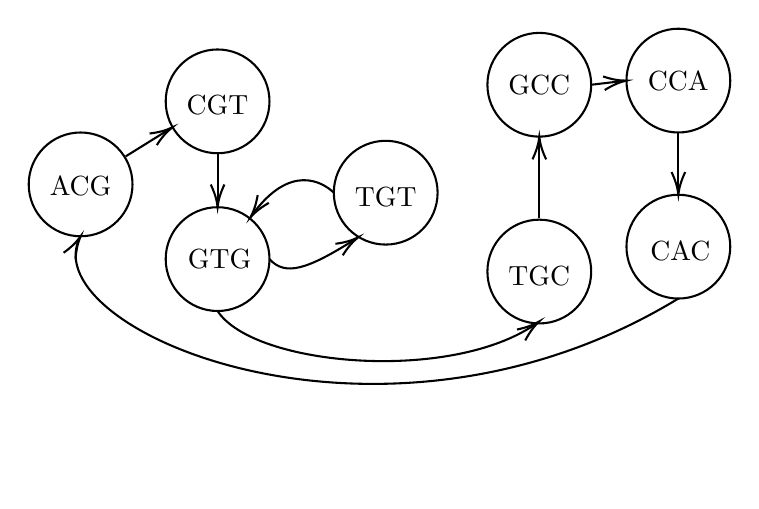
\begin{tikzpicture}[x=0.75pt,y=0.75pt,yscale=-1,xscale=1]
%uncomment if require: \path (0,248); %set diagram left start at 0, and has height of 248

%Shape: Circle [id:dp5662414203096264] 
\draw   (81,53) .. controls (81,39.19) and (92.19,28) .. (106,28) .. controls (119.81,28) and (131,39.19) .. (131,53) .. controls (131,66.81) and (119.81,78) .. (106,78) .. controls (92.19,78) and (81,66.81) .. (81,53) -- cycle ;
%Shape: Circle [id:dp13985089677551477] 
\draw   (81,129) .. controls (81,115.19) and (92.19,104) .. (106,104) .. controls (119.81,104) and (131,115.19) .. (131,129) .. controls (131,142.81) and (119.81,154) .. (106,154) .. controls (92.19,154) and (81,142.81) .. (81,129) -- cycle ;
%Shape: Circle [id:dp3574816316500795] 
\draw   (15,93) .. controls (15,79.19) and (26.19,68) .. (40,68) .. controls (53.81,68) and (65,79.19) .. (65,93) .. controls (65,106.81) and (53.81,118) .. (40,118) .. controls (26.19,118) and (15,106.81) .. (15,93) -- cycle ;
%Shape: Circle [id:dp6367614117013465] 
\draw   (162,97) .. controls (162,83.19) and (173.19,72) .. (187,72) .. controls (200.81,72) and (212,83.19) .. (212,97) .. controls (212,110.81) and (200.81,122) .. (187,122) .. controls (173.19,122) and (162,110.81) .. (162,97) -- cycle ;
%Shape: Circle [id:dp8286860889666687] 
\draw   (236,135) .. controls (236,121.19) and (247.19,110) .. (261,110) .. controls (274.81,110) and (286,121.19) .. (286,135) .. controls (286,148.81) and (274.81,160) .. (261,160) .. controls (247.19,160) and (236,148.81) .. (236,135) -- cycle ;
%Shape: Circle [id:dp04605576669499256] 
\draw   (236,45) .. controls (236,31.19) and (247.19,20) .. (261,20) .. controls (274.81,20) and (286,31.19) .. (286,45) .. controls (286,58.81) and (274.81,70) .. (261,70) .. controls (247.19,70) and (236,58.81) .. (236,45) -- cycle ;
%Shape: Circle [id:dp9155218336299027] 
\draw   (303,43) .. controls (303,29.19) and (314.19,18) .. (328,18) .. controls (341.81,18) and (353,29.19) .. (353,43) .. controls (353,56.81) and (341.81,68) .. (328,68) .. controls (314.19,68) and (303,56.81) .. (303,43) -- cycle ;
%Shape: Circle [id:dp766738912437283] 
\draw   (303,123) .. controls (303,109.19) and (314.19,98) .. (328,98) .. controls (341.81,98) and (353,109.19) .. (353,123) .. controls (353,136.81) and (341.81,148) .. (328,148) .. controls (314.19,148) and (303,136.81) .. (303,123) -- cycle ;
%Straight Lines [id:da9646625679785032] 
\draw    (61.75,79.5) -- (82.55,66.56) ;
\draw [shift={(84.25,65.5)}, rotate = 508.11] [color={rgb, 255:red, 0; green, 0; blue, 0 }  ][line width=0.75]    (10.93,-3.29) .. controls (6.95,-1.4) and (3.31,-0.3) .. (0,0) .. controls (3.31,0.3) and (6.95,1.4) .. (10.93,3.29)   ;

%Straight Lines [id:da8830983152823235] 
\draw    (106,78) -- (106,102) ;
\draw [shift={(106,104)}, rotate = 270] [color={rgb, 255:red, 0; green, 0; blue, 0 }  ][line width=0.75]    (10.93,-3.29) .. controls (6.95,-1.4) and (3.31,-0.3) .. (0,0) .. controls (3.31,0.3) and (6.95,1.4) .. (10.93,3.29)   ;

%Curve Lines [id:da7743744950450349] 
\draw    (131,129) .. controls (138.6,137.33) and (149.07,134.14) .. (172.31,119.42) ;
\draw [shift={(173.75,118.5)}, rotate = 507.41] [color={rgb, 255:red, 0; green, 0; blue, 0 }  ][line width=0.75]    (10.93,-3.29) .. controls (6.95,-1.4) and (3.31,-0.3) .. (0,0) .. controls (3.31,0.3) and (6.95,1.4) .. (10.93,3.29)   ;

%Curve Lines [id:da701157029011428] 
\draw    (162,97) .. controls (156.37,91.61) and (140.89,82.86) .. (122.86,107.45) ;
\draw [shift={(121.75,109)}, rotate = 304.92] [color={rgb, 255:red, 0; green, 0; blue, 0 }  ][line width=0.75]    (10.93,-3.29) .. controls (6.95,-1.4) and (3.31,-0.3) .. (0,0) .. controls (3.31,0.3) and (6.95,1.4) .. (10.93,3.29)   ;

%Curve Lines [id:da9534415928320956] 
\draw    (328,148) .. controls (184.94,235.12) and (18.86,163.46) .. (39.32,119.33) ;
\draw [shift={(40,118)}, rotate = 479.11] [color={rgb, 255:red, 0; green, 0; blue, 0 }  ][line width=0.75]    (10.93,-3.29) .. controls (6.95,-1.4) and (3.31,-0.3) .. (0,0) .. controls (3.31,0.3) and (6.95,1.4) .. (10.93,3.29)   ;

%Curve Lines [id:da9799576589537213] 
\draw    (106,154) .. controls (123.33,180.73) and (219.06,188.84) .. (259.78,159.89) ;
\draw [shift={(261,159)}, rotate = 503.13] [color={rgb, 255:red, 0; green, 0; blue, 0 }  ][line width=0.75]    (10.93,-3.29) .. controls (6.95,-1.4) and (3.31,-0.3) .. (0,0) .. controls (3.31,0.3) and (6.95,1.4) .. (10.93,3.29)   ;

%Straight Lines [id:da2213126680718589] 
\draw    (261,109) -- (261,72) ;
\draw [shift={(261,70)}, rotate = 450] [color={rgb, 255:red, 0; green, 0; blue, 0 }  ][line width=0.75]    (10.93,-3.29) .. controls (6.95,-1.4) and (3.31,-0.3) .. (0,0) .. controls (3.31,0.3) and (6.95,1.4) .. (10.93,3.29)   ;

%Straight Lines [id:da05405134063421202] 
\draw    (328,96) -- (328,68) ;

\draw [shift={(328,98)}, rotate = 270] [color={rgb, 255:red, 0; green, 0; blue, 0 }  ][line width=0.75]    (10.93,-3.29) .. controls (6.95,-1.4) and (3.31,-0.3) .. (0,0) .. controls (3.31,0.3) and (6.95,1.4) .. (10.93,3.29)   ;
%Straight Lines [id:da7142573004014958] 
\draw    (286,45) -- (301.01,43.23) ;
\draw [shift={(303,43)}, rotate = 533.29] [color={rgb, 255:red, 0; green, 0; blue, 0 }  ][line width=0.75]    (10.93,-3.29) .. controls (6.95,-1.4) and (3.31,-0.3) .. (0,0) .. controls (3.31,0.3) and (6.95,1.4) .. (10.93,3.29)   ;


% Text Node
\draw (40,94) node  [align=left] {ACG};
% Text Node
\draw (106,55) node  [align=left] {CGT};
% Text Node
\draw (107,129) node  [align=left] {GTG};
% Text Node
\draw (187,99) node  [align=left] {TGT};
% Text Node
\draw (261,45) node  [align=left] {GCC};
% Text Node
\draw (328,43) node  [align=left] {CCA};
% Text Node
\draw (261,137) node  [align=left] {TGC};
% Text Node
\draw (329,125) node  [align=left] {CAC};


\end{tikzpicture}
\end{center}
\end{figure}

\subsection{Cicli e cammini di Eulero}
\begin{definition}{Grafo Semi-Euleriano}{}
	Sia $G = \langle V, A \rangle$ un grafo orientato. $G$ è semi-Euleriano se esistono due vertici $s, t$ tali che $N_G^- (s) = N_G^+(s) + 1, N_G^-(t) = N_G^+(v) - 1$, mentre per ogni altro vertice $w$, $N_G^-(w) = N_G^+(w)$.
	
	Ogni nodo ha lo stesso numero di archi entranti e uscenti, tranne per due nodi di cui uno ha un arco uscente in più e l'altro uno in meno.
\end{definition}

\begin{definition}{Grafo Euleriano}{}
	Sia $G = \langle V, A \rangle $ un grafo orientato. $G$ è Euleriano se $N_G^-(w) = N_G^+(w)$, per ogni vertice (stesso numero di archi entranti e uscenti).
	\tcblower
	Sia $G = \langle V, A \rangle$ un grafo Euleriano e sia $C$ un ciclo di $G$. Sia $G_1$ il grafo ottenuto da $G$ togliendo tutti gli archi di $C$. Allora $G_1$ è Euleriano.
\end{definition}

\begin{thm}{Grafo Euleriano}{}
	Un grafo connesso $G = \langle V, A \rangle$ ha un cammino Euleriano se e solo se $G$ è semi-Euleriano. $G$ ha un ciclo Euleriano se e solo se $G$ è Euleriano.
	\tcblower
	Sia $G = \langle V, A \rangle$ un semi-Euleriano e sia $P$ un cammino da $s$ a $t$. Sia $G_1$ il grafo ottenuto da $G$ togliendo tutti gli archi di $P$. Allora $G_1$ è Euleriano.
\end{thm}

\begin{definition}{Ciclo Euleriano e Hamiltoniano}{}
	Un ciclo (cammino) Euleriano è un assemblaggio in un grafo orientato e connesso che attraversa ogni \textbf{arco} esattamente una volta.
	\tcblower
	Un ciclo Hamiltoniano (caso particolare di TSP) è un cammino che attraversa ogni \textbf{vertice} esattamente una volta.
\end{definition}

Il primo problema è risolvibile con un algoritmo in tempo lineare, mentre il secondo è NP-completo. 

Un ciclo viene chiamato semplice se non tocca due volte lo stesso vertice: è possibile trovare cicli Euleriani in questi casi, ma non ci saranno cicli Hamiltoniani. 

L'algoritmo è in tempo lineare: ciò significa che per ogni arco si spende un tempo costante. Si parte dal primo vertice, e si prosegue verso un arco uscente $s$. Si cercano sempre archi uscenti che non sono già stati visitati, e si termina quando non ne esistono più.

L'ultimo vertice è la destinazione, che ha un numero di archi entranti superiore di 1 rispetto agli archi uscenti. Togliendo il cammino Euleriano, il grafo diventa sicuramente Euleriano (formato da un insieme di cicli), anche se non necessariamente connesso. 

Ci dev'essere un vertice toccato dal cammino Euleriano che ha un arco uscente non ancora visitato. Come prima, si guarda quest'ultimo arco del vertice, e la procedura termina nello stesso di partenza: si è trovato un altro ciclo. 

I vari cicli, dopo essere stati trovati, vengono ricombinati.

\subsection{Reverse and complement}
All'algoritmo precedente viene aggiunta una complicazione: non si conosce lo strand di DNA. La stessa stringa potrebbe aver subito un reverse and complement, e non si sa quale delle due possibilità è effettivamente quella corretta.

Per evitare il raddoppio dello spazio di memoria, si indica la read canonica come la prima in ordine lessicografico, però a ogni calcolo dell'overlap viene considerato anche il complemento.

L'idea di base è che i valori più lunghi di $k$ sono più espressivi, perché permettono di gestire meglio le sovrapposizioni. I numeri dispari sono migliori, perché altrimenti potrebbero esistere $k$-meri che hanno reverse and complement uguali all'originale. 

Il genoma è diploide (copie quasi perfettamente identiche), ma le differenze formano percorsi separati in un grafo chiamato \textit{bolla} (\textbf{bubble popping}). La lunghezza dei percorsi è variabile, e alcuni di essi non portano da nessuna parte: vengono rimossi in un processo chiamato \textbf{tip removal}. Attraverso questo perfezionamento delle sequenze sono costruiti i contig.

Un'altra fase importante è, dato un frammento del DNA di origine, capire se ci sono match tra contigs per poterli inserire in porzioni adiacenti (perché sono diploidi). Non sono ancora conosciuti tutti i possibili match.